%! TEX program = xelatex
\documentclass[12pt]{report}

\usepackage[utf8]{inputenc}
\usepackage{geometry}
\usepackage{graphicx}
\usepackage{fontspec}
\usepackage{fancyhdr}
\usepackage{setspace}
\usepackage{blindtext}
\usepackage{titlesec}
\usepackage{multirow}
\usepackage{changepage}
\usepackage{array}
\usepackage{float}
\usepackage{longtable}
\usepackage{tabularx}
\usepackage{pgffor}
\usepackage{amsmath}
\usepackage{caption}
\usepackage{subcaption}
\usepackage{hyperref}
\usepackage{listings}
\usepackage{xcolor}
\usepackage[backend=biber,style=authoryear]{biblatex}
\addbibresource{citations/citation.bib}

% add image paths
\graphicspath{{images/}}

\newenvironment{subs}
  {\adjustwidth{3em}{0pt}}
  {\endadjustwidth}

  \lstset{
    language=Python,
    basicstyle=\ttfamily\scriptsize, % Tiny font to prevent overflow
    keywordstyle=\color{blue}\bfseries,
    stringstyle=\color{red},
    commentstyle=\color{green!60!black},
    backgroundcolor=\color{gray!10},
    frame=single,
    breaklines=true, % Enable line wrapping
    breakatwhitespace=true, % Break lines at spaces or tabs
    xleftmargin=0pt, % Add left margin
    xrightmargin=2em, % Add right margin
    showstringspaces=false,
    columns=fullflexible, % Ensure proper alignment
    aboveskip=1em,
    belowskip=1em,
    linewidth=\textwidth,  % Ensure the code block fits within the page width
    escapeinside={(*@}{@*)},  % To include latex commands in code (if needed)
    keepspaces=true,  % Ensure spaces in the code are respected
    showtabs=false,  % Hide tabs
    tabsize=4,  % Set tab size for indentation
  }

% set layout
\geometry{
 a4paper,
 tmargin=4cm,
 bmargin=3cm,
 lmargin=4cm,
 rmargin=3cm,
}

% Change default naming
\renewcommand{\figurename}{Gambar}
\renewcommand{\contentsname}{Daftar Isi}

% set title spacing and change main font family
\titlespacing*{\chapter}{0pt}{18pt plus 6pt minus 6pt}{6pt}
\titlespacing*{\section}{0pt}{18pt plus 6pt minus 6pt}{6pt}
\titlespacing*{\subsection}{0pt}{18pt plus 6pt minus 6pt}{6pt}
\setmainfont{Times New Roman}

% add title page
\title{ANALISIS PERGERAKAN HARGA SAHAM DI INDONESIA SEBAGAI SISTEM PENDUKUNG KEPUTUSAN INVESTASI BERDASARKAN DATA HISTORIS DENGAN ALGORITMA LONG SHORT-TERM MEMORY (LSTM)}
\author{Ilham Suandi \\ Information Systems}
\date{}

% begin document
\begin{document}
% set word wrap and hyphenation
\hyphenpenalty=10000
\exhyphenpenalty=10000
\setlength{\emergencystretch}{2em}

% set paragraph spacing
\onehalfspacing
\frenchspacing

% set paragraph indentation
\setlength{\parindent}{1cm}

% TODO: hapus nomor halaman pada title page
% add title page
\begin{titlepage}
	\thispagestyle{empty}
	\titleformat{\chapter}[hang]{\fontsize{14}{14}\centering\bfseries}{\thechapter}{}{}
	\titleformat{\section}[hang]{\fontsize{14}{14}\bfseries\centering}{\textbf{\thesection}}{1pc}{}
	\centering
	\chapter*{SKRIPSI}
	\section*{ANALISIS PERGERAKAN HARGA SAHAM DI INDONESIA SEBAGAI SISTEM PENDUKUNG KEPUTUSAN INVESTASI BERDASARKAN DATA HISTORIS DENGAN ALGORITMA LONG SHORT-TERM MEMORY (LSTM)}
	\vspace{2cm}
	Diajukan untuk Memenuhi Salah Satu Syarat Memperoleh Gelar Sarjana
	\begin{figure}[H]
		\centering
		
\includegraphics[width=0.4\textwidth]{logo_unas.png}
	\end{figure}
	\textbf{ILHAM SUANDI ARDI WINATA} \\
	\textbf{217006516020} \\
	\vfill
	{\fontsize{14}{16}\selectfont \textbf{PROGRAM STUDI INFORMATIKA}} \\
	{\fontsize{13}{16}\selectfont \textbf{FAKULTAS TEKNOLOGI KOMUNIKASI DAN INFORMATIKA}} \\
	{\fontsize{13}{16}\selectfont \textbf{UNIVERSITAS NASIONAL}} \\
	{\fontsize{13}{16}\selectfont \textbf{JAKARTA}} \\
	{\fontsize{13}{16}\selectfont \textbf{2024}}
\end{titlepage}

% Add List of Figures and Tables to the Table of Contents
\pagenumbering{roman}

\titleformat{\chapter}[hang]{\fontsize{14}{14}\centering\bfseries}{\thechapter}{}{}
\chapter*{LAMPIRAN PERSETUJUAN}
\pagebreak

\titleformat{\section}[hang]{\fontsize{12}{12}\bfseries\centering}{\textbf{\thesection}}{1pc}{}
\chapter*{ANALISIS PERGERAKAN HARGA SAHAM DI INDONESIA SEBAGAI SISTEM PENDUKUNG KEPUTUSAN INVESTASI BERDASARKAN DATA HISTORIS DENGAN ALGORITMA LONG SHORT-TERM MEMORY (LSTM)}
\vspace{2cm}
\section*{SKRIPSI}
\vspace{2cm}
\begin{center}
	Diajukan kepada:\\
	Universitas Nasional Jakarta \\
	Untuk memenuhi Salah Satu Persyaratan dalam \\
	Memperoleh Gelar Sarjana Komputer (S.Kom) \\
	\vspace{2cm}
	\textbf{Oleh:}\\
	\textbf{Ilham Suandi Ardi Winata}\\
	\textbf{NIM: 217006516020}\\
	\vfill
	{\fontsize{14}{16}\selectfont \textbf{PROGRAM STUDI INFORMATIKA}} \\
	{\fontsize{13}{16}\selectfont \textbf{FAKULTAS TEKNOLOGI KOMUNIKASI DAN INFORMATIKA}} \\
	{\fontsize{13}{16}\selectfont \textbf{UNIVERSITAS NASIONAL}} \\
	{\fontsize{13}{16}\selectfont \textbf{JAKARTA}} \\
	{\fontsize{13}{16}\selectfont \textbf{2024}}
\end{center}
\pagebreak

\chapter*{HALAMAN PENGESAHAN}
\pagebreak

\chapter*{PERNYATAAN KEASLIAN TULISAN}
\pagebreak

\chapter*{KATA PENGANTAR}
\vspace{0.5cm}
\indent

Segala puji hanya milik Allah Subhanahu Wa Ta’ala atas segala nikmat dan kasih sayang Nya yang telah memudahkan penulis untuk menyelesaikan skripsi yang berjudul “ ANALISIS PERGERAKAN HARGA SAHAM DI INDONESIA SEBAGAI SISTEM PENDUKUNG KEPUTUSAN INVESTASI BERDASARKAN DATA HISTORIS DENGAN ALGORITMA LONG SHORT-TERM MEMORY (LSTM) ”. Semoga shalawat dan salam senantiasa terlimpah kepada Nabi Muhammad Sallalahu ‘Alaihi wa Sallam. Dan semoga kita semua mendapat syafaatnya di hari kiamat nanti, Aamiin.
\vspace{0.5cm}

Penulis mengucapkan rasa syukur dan terima kasih yang tak terhingga kepada semua pihak-pihak yang selalu memberikan bantuan dan motivasi kepada penulis untuk dapat menyelesaikan skripsi ini. Ucapan ini penulis sampaikan kepada:

\begin{enumerate}
	\item Rektor
	\item Dospem
	\item KAPRODI
	\item Dospem 1\&2
	\item Orang Tua
\end{enumerate}

Akhir kata, penulis mengakui bahwa penulisan pada skripsi ini masih banyak kekurangan. Saya berharap semoga skripsi ini diterima sebagai amal ibadah yang tulus dan bermanfaat di sisi Allah Subhanahu Wa Ta’ala. Semoga karya ini menjadi bagian dari kontribusi yang tak terputus dalam rangka memperkuat dan mengembangkan ilmu pengetahuan, serta melaksanakan tugas sebagai manusia yang berkomitmen.

\vfill
{\raggedleft
	Jakarta, 22 September 2024
	\par}
\pagebreak

% set default title format
\titleformat{\chapter}[hang]{\fontsize{12}{12}\centering\bfseries}{\thechapter}{}{}
\titleformat{\section}[hang]{\fontsize{12}{12}\bfseries}{\textbf{\thesection}}{1pc}{}
\titleformat{\subsection}[hang]{\fontsize{12}{12}\bfseries}{\thesubsection}{1pc}{}
\titleformat{\subsubsection}[hang]{\fontsize{12}{12}\bfseries}{\thesubsubsection}{1pc}{}

% Table of Contents
% TODO: tambahkan hyperref untuk seluruh item yang ada didalam TOC
\tableofcontents
\addcontentsline{toc}{chapter}{Daftar Isi}

\newpage

% Start Arabic numbering from here
\pagenumbering{arabic}

% chapter 1
\setcounter{chapter}{1}
\chapter*{\textbf{BAB I \\ PENDAHULUAN}}
\addcontentsline{toc}{chapter}{BAB I}
\addcontentsline{toc}{chapter}{PENDAHULUAN}

\textbf{\section{LATAR BELAKANG}}
\indent

Pasar saham merupakan salah satu instrumen investasi yang sangat menarik bagi para investor dikarenakan keuntungan saham yang jauh lebih besar dibanding instrumen investasi lainnya (\cite{Shen2020}). Namun saham juga memiliki resiko yang sangatlah tinggi dibanding instrumen investasi lainnya. Fluktuasi harga saham yang sering terjadi di pasar saham membuat investor perlu strategi dan keputusan yang tepat untuk meminimalisir resiko adn memaksimalkan keuntungan. Dengan adanya teknologi analisis data, maka dapat dilakukan prediksi berdasarkan data historical. Salah satu algoritma yang cocok untuk mengolah data historical adalah \textit{LONG SHORT-TERM MEMORY} (LSTM). \textit{LSTM} merupakan sebuah algoritma pembelajaran mendalam (deep learning) yang mampu menangkap pola temporal dalam data historical. Dengan analisis ini dapat memudahkan investor dalam pengambilan keputusan investasi.

Dalam beberapa dekade terkahir ini perkembangan teknologi terutama pada bidang kecerdasan buatan. Kecerdasan buatan telah berkontribusi besar pada sektor analisis dan pengolahan data keuangan. Salah satu pendekatan yang terkenal sangat efektif adalah \textit{LONG SHORT-TERM MEMORY} (LSTM). Algoritma ini mampu menangkap pola temporal pada data time series, sehingga cocok untuk memprediksi harga saham yang cenderung bersifat dinamis dan non-linear (\cite{chairurrachman2022penerapan}).

Penelitian ini akan menggunakan data historis yang akan dikumpulkan menggunakan emiten atau perusahaan Indonesia yang terdapat pada \textit{Yahoo Finance} yang tentu saja terdaftar juga pada Bursa Efek Indonesia (BEI) (\cite{julian2021peramalan}). Data ini akan dikumpulkan menggunakan \textit{Python} dan \textit{Pandas} untuk mengolah data. Data yang dikumpulkan akan dikumpulkan menggunakan algoritma \textit{LSTM} yang akan digunakan untuk memprediksi harga saham pada bursa efek Indonesia. Data yang dikumpulkan akan dikumpulkan menggunakan algoritma \textit{LSTM} yang akan digunakan untuk memprediksi harga saham pada bursa efek Indonesia.

\pagebreak

\textbf{\section{Rumusan Masalah}}
\noindent
Rumusan masalah yang ada dalam penelitian ini adalah: 
\begin{enumerate}
    \item Bagaimana pola pergerakan harga saham di Indonesia dapat di analisis secara efektif menggunakan data historis untuk mendukung pengambilan keputusan investasi? 
    \item Bagaimana sistem pendukung keputusan berbasis algoritma LSTM dapat membantu investor dalam membuat keputusan investasi yang lebih terinformasi di pasar saham Indonesia?
\end{enumerate}

\textbf{\section{Tujuan Penelitian}}
\noindent
Tujuan dari penelitian ini adalah untuk:

\begin{enumerate} 
  \item Menganalisis pola pergerakan harga saham di Indonesia berdasarkan data historis
  \item Mengembangkan sistem pendukung keputusan berbasis algoritma LSTM untuk membantu investor
\end{enumerate} 

\textbf{\section{Manfaat Penelitian}}
\noindent
Adapun beberapa manfaat dari penelitian ini adalah:

\begin{enumerate} 
  \item Membantu investor dalam mengambil keputusan investasi berbasis data
  \item Mengembangkan literatur tentang penerapan LSTM dalam prediksi saham di Indonesia

\end{enumerate} 

\textbf{\section{Batasan Masalah}}

Untuk menjaga fokus dari penelitian ini, penelitian ini memiliki beberapa batasan masalah yang harus diperhatikan. Berikut ini adalah batasan masalah yang harus diperhatikan:

\begin{enumerate}
	\item Sumber Data \\
	      Data yang digunakan dalam penelitian ini hanya berasal dari Yahoo Finance, yang mencakup harga saham historis yang terdaftar di Bursa Efek Indonesia (BEI). Penelitian ini tidak mencakup data dari sumber lain seperti laporan tahunan perusahaan atau data ekonomi makro yang mungkin relevan untuk analisis saham.

	\item Jenis Saham \\
	      Penelitian ini fokus pada saham-saham yang terdaftar dalam Bursa Efek Indonesia (BEI) yaitu LQ45.

	\item Rentang Waktu \\
	      Data historis yang digunakan dalam penelitian ini terbatas pada periode 5 hingga 10 tahun terakhir. Penelitian tidak mencakup analisis harga saham yang lebih lama atau data yang sangat baru (misalnya dalam beberapa bulan terakhir), yang dapat dipengaruhi oleh kondisi pasar yang sangat volatil atau kejadian luar biasa.

	\item Fokus Model Prediksi \\
	      Model yang digunakan dalam penelitian ini adalah algoritma Long Short-Term Memory (LSTM) yang hanya memanfaatkan data harga saham historis (OHLC dan volume perdagangan) tanpa mempertimbangkan faktor fundamental lain seperti laporan keuangan perusahaan, berita pasar, atau faktor eksternal lainnya.

	\item Jenis Keputusan Investasi \\
	      Penelitian ini hanya akan menghasilkan rekomendasi investasi berupa membeli, menjual, atau menahan saham berdasarkan prediksi pergerakan harga yang dihasilkan oleh model LSTM. Penelitian tidak mencakup analisis lebih lanjut tentang strategi investasi atau manajemen portofolio.

	\item Implementasi Sistem Pendukung Keputusan \\
	      Penelitian ini fokus pada penggunaan hasil prediksi LSTM sebagai dasar rekomendasi investasi, tanpa mengembangkan sistem pendukung keputusan yang lebih kompleks atau menyertakan pengambilan keputusan berbasis faktor eksternal atau keputusan multi-parameter.
\end{enumerate}


% chapter 2
\setcounter{chapter}{2}
\setcounter{section}{0}
\chapter*{\textbf{BAB II \\ KAJIAN PUSTAKA}}
\addcontentsline{toc}{chapter}{BAB II}
\addcontentsline{toc}{chapter}{KAJIAN PUSTAKA}

\section{Landasan Teori}
\indent

Hasil dari penelitian ini adalah melakukan analisis pergerakan harga saham dan prediksi harga saham di masa yang akan datang dengan menggunakan \textit{Deep Learning}. Deep learning merupakan sebuah konsep kecerdasan buatan yang menggunakan jaringan saraf tiruan untuk memahami serta mempelajari data mulai dari data yang sederhana hingga data yang kompleks. Dengan demikian, proses analisis data saham akan jauh lebih efisien dibandingkan dengan melakukan prosesnya secara manual.

% TODO: ganti referensinya
Algoritma yang akan digunakan untuk melakukan analisis ini adalah \textit{Long Short-Term Memory (LSTM)}. Dengan algoritma ini, memungkinkan model untuk meraih tingkat akurasi yang lebih tinggi dibandingkan dengan model dengan algoritma lain. Dengan akurasi yang lebih tinggi, tentunya akan memudahkan pengguna ataupun investor untuk melakukan analisis dan membantu dalam pengambilan keputusan investasi. Selain itu algoritma LSTM juga dapat mencegah terjadinya permasalahan yang sering terjadi pada saat melakukan proses analisis data saham, yaitu \textit{vanishing gradient} (\cite{sofi2021perbandingan}).

\begin{subs}
	\textbf{\subsection{Saham}}
	% TODO: ganti referensinya
	Investasi merupakan suatu kegiatan penanaman modal berupa uang ataupun harta dengan harapan untuk  mendapatkan keuntungan di masa yang akan datang. Saham merupakan salah satu instrumen investasi yang sangat menarik bagi para investor karena potensi keuntungan yang lebih besar dibandingkan dengan investasi lainnya seperti obligasi dan deposito. Namun perlu diperhatikan bahwa sesuatu yang memiliki keuntungan lebih besar tentunya memiliki risiko yang lebih tinggi juga. Saham seringkali mengalami fluktuasi harga yang membuat saham merupakan investasi dengan risiko yang tinggi. Fluktuasi biasanya dipengaruhi oleh beberapa faktor seperti, kondisi ekonomi internal perusahaan ataupun eksternal, sentimen pasar, serta peristiwa politik maupun sosial lainnya (\cite{Rosyd2024PENERAPANML}).

	\begin{figure}[H]
		\centering
		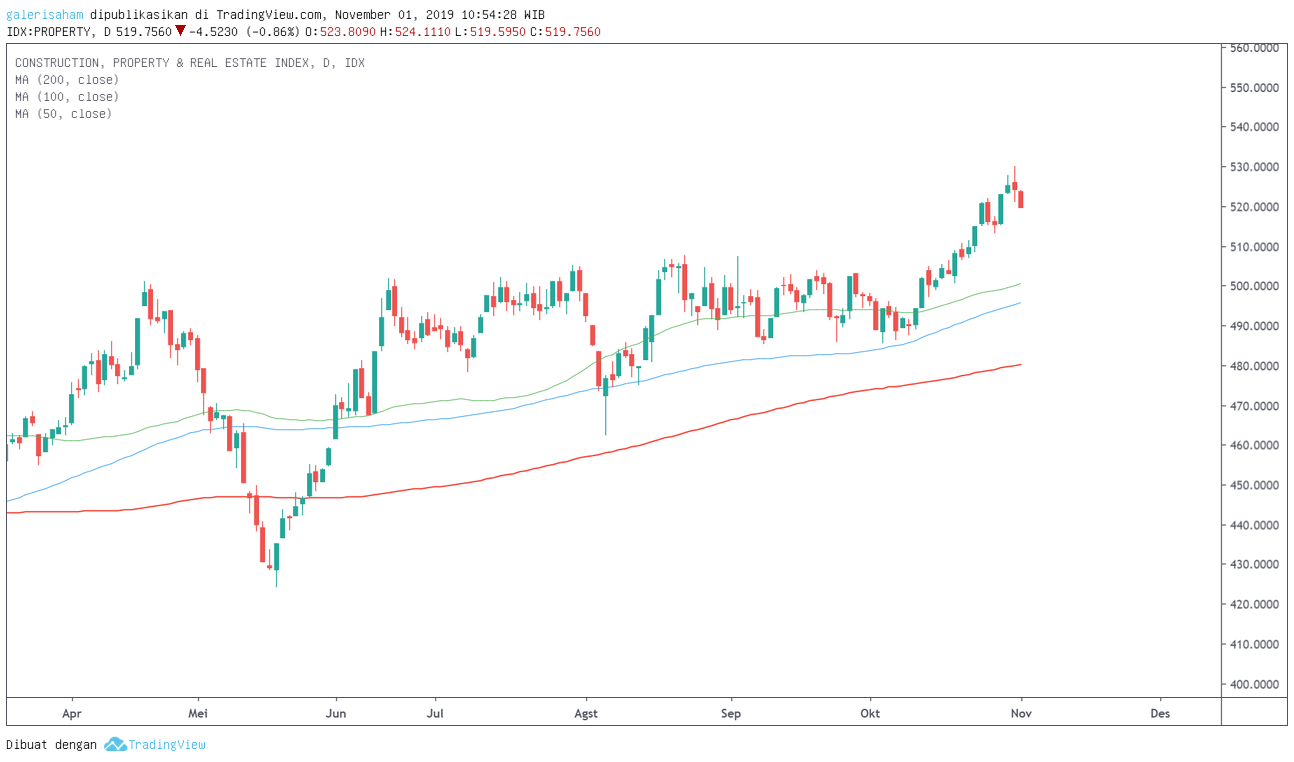
\includegraphics[width=0.8\textwidth]{chart_saham.png}
		\caption{Fluktuasi Harga Saham}
	\end{figure}

	Saham atau pasar modal merupakan sebuah sertifikat/surat yang berharga yang menunjukkan kepemilikan atas suatu perusahaan, dalam sertifikat tercantum nilai saham yang dimiliki, jenis saham yang dimiliki, hak dan kewajiban setiap pemegang saham (\cite{ChristianANALISIS}). Jadi saham merupakan sebuah surat berharga yang menandakan kepemilikan atas suatu perusahaan. Sebagai pemegang saham investor memiliki hak untuk memperoleh hak untuk menerima dividen, hak suara dalam rapat umum pemegang saham dan juga keuntungan dari kenaikan harga saham (\cite{MerissaKeuntunganSaham}).

	Tujuan utama dari investasi saham adalah untuk menghasilkan keuntungan di masa yang akan datang. Artinya investor membeli saham dengan harapan harga saham akan meningkat di masa yang akan datang (\textit{Capital Gain}) yang tentunya menguntungkan investor. Selain dari itu, investasi saham juga dapat memberikan pendapatan pasif (\textit{Pasive Income}) kepada investor yang berupa dividen. Keuntungan dari saham terbagi menjadi dua yaitu, pendapatan dividen dan pertumbuhan saham (\textit{Capital Gain}). Dividen merupakan keuntungan bersih dari perusahaan yang akan dibagikan kepada para pemegang sahamnya. Namun, tidak semua perusahaan membagikan dividen kepada para investor.

	Dengan keuntungan yang tinggi tentunya memilih saham memerlukan beberapa teknik analisis, yaitu analisis fundamental dan juga analisis teknikal. Analisis fundamental merupakan sebuah teknik analisa yang memperhitungkan faktor fundamental sebuah perusahaan yang dapat memengaruhi pergerakan harga saham. Faktor-faktor fundamental ini meliputi, kondisi ekonomi perusahaan, dalam negeri maupun luar negeri, tren pasar/tren industri juga termasuk kedalam faktor fundamental, tingkat persaingan perusahaan, dan juga kebijakan fiskal dan moneter serta yang paling utama yaitu faktor kinerja dari perusahaan yang dapat dicek melalui catatan/laporan keuangan perusahaan tersebut. Selain itu analisis teknikal juga memainkan peran penting dalam memilih saham. analisis teknikal merupakan teknik analisis dengan menggunakan data historis terkait saham seperti menganalisa pergerakan harga saham masa lalu untuk memprediksi harga saham yang akan terjadi di masa depan.
\end{subs}

\begin{subs}
	\textbf{\subsection{Saham LQ45}}
	Indeks LQ45 adalah salah satu indeks saham di Bursa Efek Indonesia (BEI) yang terdiri dari 45 saham yang dipilih berdasarkan kriteria likuiditas dan kapitalisasi pasar yang tinggi. Indeks ini mencakup saham-saham dari perusahaan-perusahaan terkemuka di Indonesia yang dianggap memiliki stabilitas dan daya saing tinggi, serta memainkan peran penting dalam perekonomian Indonesia. Saham-saham dalam LQ45 merupakan representasi dari perusahaan dengan kinerja terbaik dan sering kali menjadi acuan bagi para investor domestik maupun internasional. Saham-saham yang terdaftar dalam LQ45 mencakup berbagai sektor industri seperti perbankan, energi, infrastruktur, dan konsumsi, yang menunjukkan keberagaman sektor yang ada di Indonesia (\cite{kusuma2020saham}).

	Salah satu karakteristik utama dari saham LQ45 adalah likuiditasnya yang tinggi. Saham dengan likuiditas tinggi lebih mudah diperdagangkan karena memiliki volume transaksi yang besar, yang memberikan keuntungan bagi investor dalam hal kemudahan transaksi serta potensi pergerakan harga yang lebih terprediksi. Selain itu, saham-saham dalam LQ45 sering menjadi pilihan utama bagi investor institusional dan fund manager karena saham-saham tersebut dianggap lebih stabil dan cenderung memiliki risiko lebih rendah dibandingkan dengan saham-saham lain di pasar saham Indonesia (\cite{wibowo2018analisis}).

	Pergerakan harga saham dalam LQ45 dapat digunakan untuk menggambarkan kondisi pasar saham Indonesia secara keseluruhan. Oleh karena itu, saham-saham dalam indeks ini sering dianalisis menggunakan berbagai pendekatan, baik itu analisis teknikal maupun analisis fundamental. Dalam analisis teknikal, investor menggunakan berbagai indikator seperti Moving Average (MA), Relative Strength Index (RSI), dan Bollinger Bands untuk mengidentifikasi tren pasar dan memprediksi pergerakan harga saham di masa depan. Sementara itu, dalam analisis fundamental, faktor-faktor yang dianalisis meliputi laporan keuangan perusahaan, manajemen perusahaan, serta faktor makroekonomi yang dapat mempengaruhi kinerja perusahaan-perusahaan yang terdaftar dalam LQ45 (\cite{hutagalung2019analisis}).

	Selain itu, dengan semakin berkembangnya teknologi, terutama dalam bidang kecerdasan buatan, penelitian terkait analisis saham LQ45 mulai mengarah pada penggunaan algoritma machine learning, termasuk deep learning. Salah satu algoritma yang banyak digunakan dalam penelitian ini adalah Long Short-Term Memory (LSTM). LSTM memiliki kemampuan untuk menangani data deret waktu (time series) yang bersifat dinamis dan non-linear, seperti halnya pergerakan harga saham yang sering mengalami fluktuasi. Beberapa penelitian menunjukkan bahwa LSTM lebih efektif dibandingkan dengan model-model lain, seperti Recurrent Neural Networks (RNN), dalam memprediksi pergerakan harga saham (\cite{chairurrachman2022penerapan}; \cite{alim2023pemodelan}). Keunggulan LSTM terletak pada kemampuannya untuk mengatasi masalah vanishing gradient, sehingga lebih efisien dalam melakukan prediksi harga saham berdasarkan data historis.

  Dengan meningkatnya ketertarikan investor untuk menggunakan teknologi dalam analisis pasar saham, LQ45 menjadi salah satu indeks yang sering dianalisis menggunakan metode-metode canggih seperti LSTM. Ini memberikan peluang bagi investor untuk memperoleh informasi yang lebih akurat dan terpercaya, yang pada gilirannya dapat membantu mereka dalam membuat keputusan investasi yang lebih baik dan menguntungkan (\cite{pipin2023deep}).
\end{subs}


\begin{subs}
	\textbf{\subsection{Kecerdasan Buatan}}
	Kecerdasan buatan atau yang lebih biasa dikenal sebagai \textit{Artificial Intelligence} (AI) merupakan teknik yang memungkinkan komputer untuk memahami dan memproses data. \textit{Artificial Intelligence} (AI) merupakan teknik komputer yang memiliki kemampuan untuk menganalisis data dan menemukan solusi untuk masalah yang ada. \textit{Artificial Intelligence} merupakan teknik komputer yang dapat mengambil keputusan dari data yang dikumpulkan. \textit{Artificial Intelligence} memiliki kemampuan untuk menganalisis data, menemukan solusi dan menghasilkan hasil yang relevan (\cite{suleimenov2020artificial}).
	\begin{figure}[H]
		\centering
		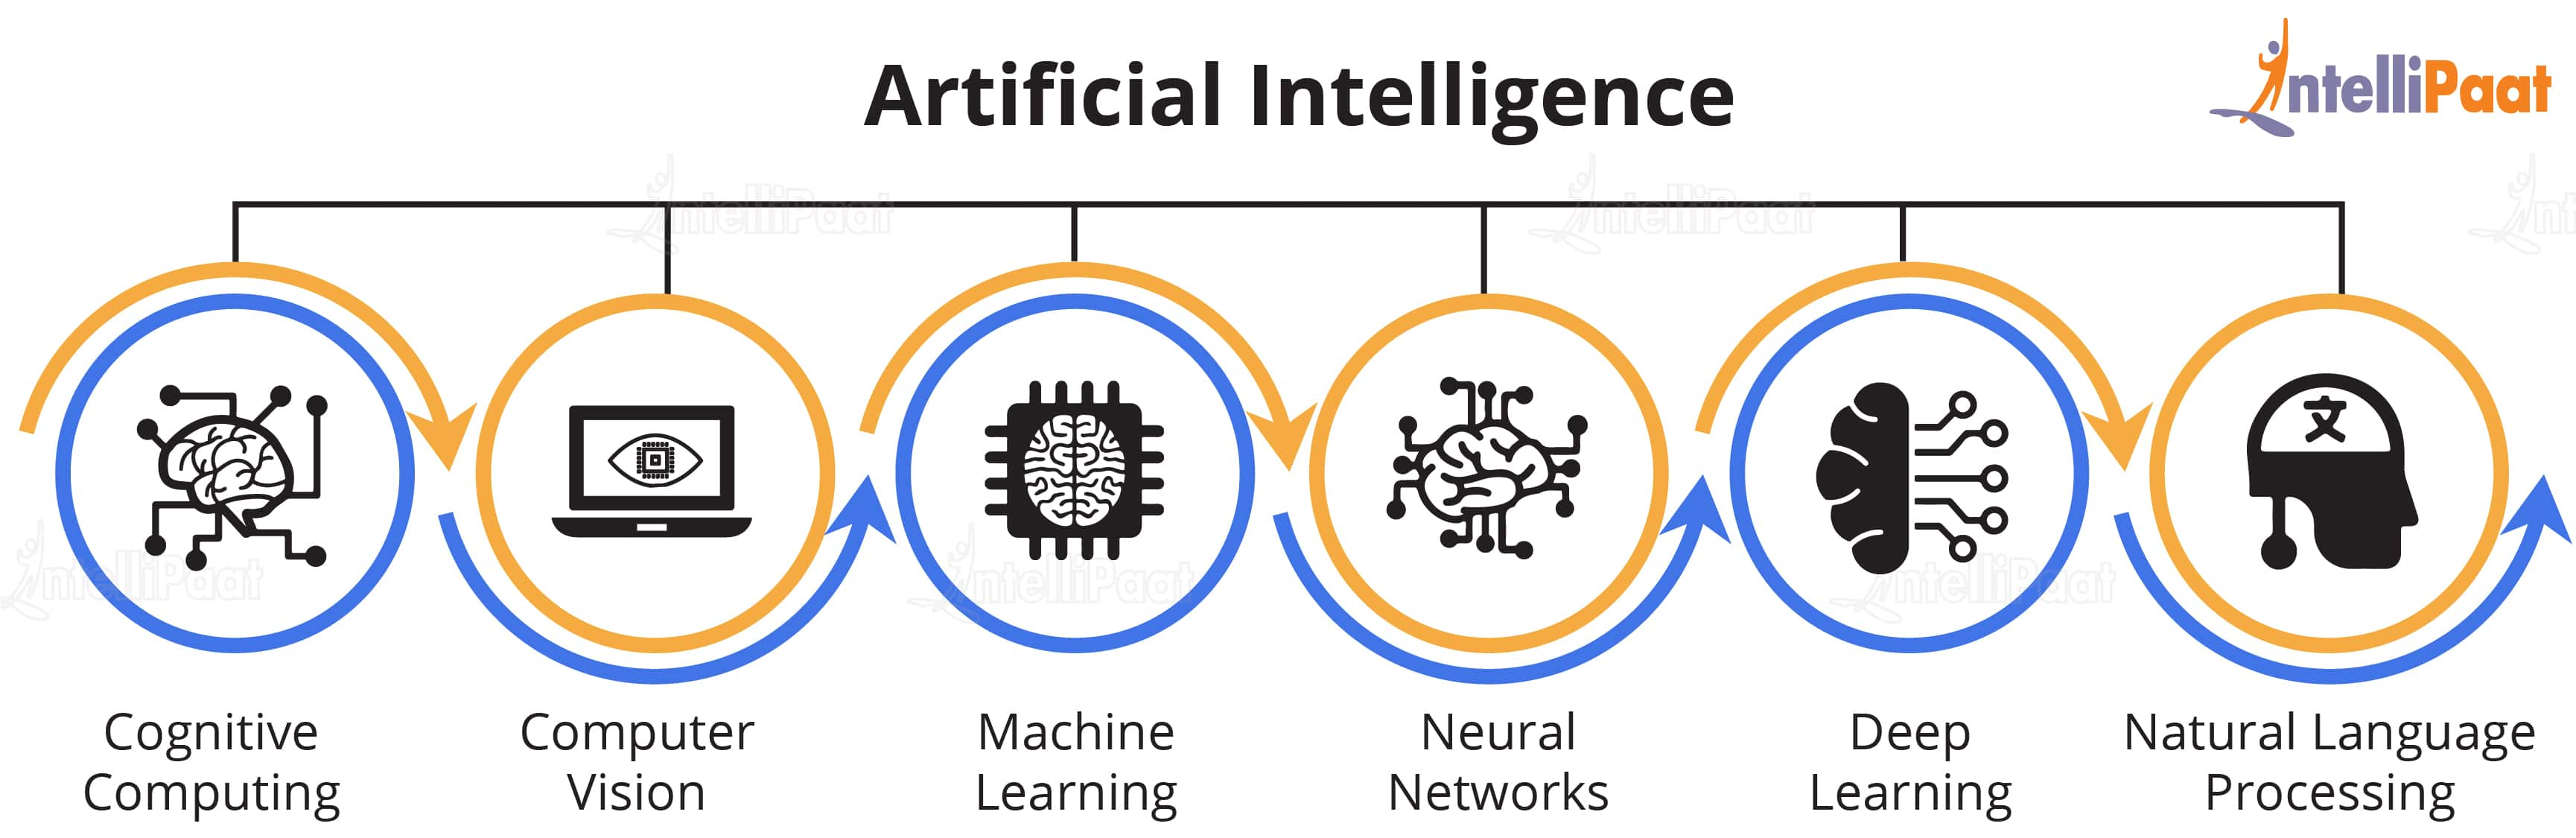
\includegraphics[width=0.8\textwidth]{artificial intelligence.jpg}
		\caption{Pendekatan Kecerdasan Buatan}
	\end{figure}
	Kecerdasan buatan dibuat untuk berfokus untuk melakukan pekerjaan yang biasanya membutuhkan kecerdasan dari manusia. Dengan itu Kecerdasan buatan dibuat guna untuk mempermudah manusia dalam menyelesaikan tugas-tugas/pekerjaan sehari-hari. Ada beberapa pendekatan dalam kecerdasan buatan yaitu,
	% TODO: benerin lagi 20
	\begin{itemize}
		\item Cognitive Computing (Komputasi Kognitif) \\
		      Komputasi kognitif adalah teknologi yang bertujuan untuk meniru cara otak manusia bekerja. Teknologi ini menggabungkan berbagai teknik seperti pembelajaran mesin, pemrosesan bahasa alami, dan analisis data untuk menciptakan sistem yang dapat memahami, bernalar, belajar, dan berinteraksi dengan manusia secara alami. Contohnya adalah IBM Watson, yang mampu menganalisis data dan memberikan wawasan seperti manusia.
		\item Computer Vision (Pengenalan Gambar) \\
		      Computer vision adalah cabang kecerdasan buatan yang berfokus pada bagaimana komputer dapat memahami dan menafsirkan dunia visual, seperti gambar dan video. Teknologi ini digunakan dalam berbagai aplikasi seperti pengenalan wajah, deteksi objek, dan analisis video. Algoritma dalam computer vision memproses gambar dengan cara yang mirip manusia mengenali pola visual.
		\item Machine Learning (Pembelajaran Mesin) \\
		      Machine learning adalah teknik yang memungkinkan sistem komputer belajar dari data tanpa pemrograman eksplisit. Dalam metode ini, algoritma dilatih menggunakan dataset untuk mengenali pola, membuat prediksi, atau mengambil keputusan. Contohnya termasuk rekomendasi produk di e-commerce atau deteksi email spam. Teknologi ini dianggap dasar dalam kecerdasan buatan modern.
		\item Neural Network (Jaringan Saraf Tiruan ) \\
		      Neural network adalah model komputasi yang terinspirasi oleh cara kerja otak manusia, terdiri dari neuron buatan yang terhubung satu sama lain dalam lapisan. Jaringan ini digunakan untuk memproses data kompleks, seperti mengenali pola dalam gambar atau memahami bahasa alami. Contoh penerapannya adalah dalam sistem pengenalan suara dan pemrosesan gambar.
		\item Deep Learning (Pembelajaran Mendalam ) \\
		      Deep learning adalah cabang dari machine learning yang menggunakan jaringan saraf tiruan dengan banyak lapisan (deep neural networks). Teknologi ini dirancang untuk menganalisis data besar dan kompleks, seperti gambar, teks, atau suara, dan menghasilkan prediksi atau keputusan yang lebih akurat. Contoh penerapan deep learning adalah dalam mobil otonom untuk mengenali lingkungan sekitarnya.
		\item Natural Language Processing (Pengenalan Bahasa Alami ) \\
		      Natural Language Processing (NLP) adalah teknologi yang memungkinkan komputer memahami, menganalisis, dan menghasilkan bahasa manusia. Aplikasi dari NLP meliputi asisten virtual seperti Siri atau Alexa, penerjemahan mesin, dan chatbot. Teknologi ini membantu komputer berinteraksi dengan manusia dalam bahasa alami yang digunakan sehari-hari.
	\end{itemize}
\end{subs}

% TODO: masih belum sempurna karena kesempurnaan hanya milik tuhan
% TODO: ganti referensinya
\begin{subs}
	\textbf{\subsection{Python}}
	\begin{figure}[H]
		\centering
		
\includegraphics[width=0.4\textwidth]{python.jpg}
		\caption{Python}
	\end{figure}
	Python merupakan bahasa pemrograman modern dan juga populer yang sering digunakan untuk melakukan pengembangan kecerdasan buatan, termasuk LSTM yang merupakan sebuah model \textit{deep learning}. Python memiliki fitur yang memungkinkan pengguna untuk membuat \textit{script} yang dapat dijalankan secara otomatis. Python merupakan bahasa pemrograman high level yang dimana \textit{syntax}-nya mendekati bahsasa manusia. Python juga memiliki fitur yang memungkinkan pengguna untuk membuat \textit{library} yang dapat digunakan oleh \textit{script} lain untuk mempermudah proses pembuatan aplikasi. Selain itu Python juga memiliki fitur yang memungkinkan pengguna untuk mengakses \textit{package} yang berhubungan dengan \textit{library} tersebut. Dengan demikian, Python dapat digunakan untuk melakukan analisis data saham yang menggunakan LSTM .
	Python memiliki banyak sekali \textit{Library} yang sangat mendukung untuk melakukan pengembangan kecerdasan buatan termasuk LSTM. Dengan demikian, pengguna akan lebih mudah untuk melakukan pembuatan aplikasi kecerdasan buatan yang lebih kompleks. LSTM adalah varian dari jaringan saraf tiruan (Recurrent Neural Networks, RNN) yang dirancang untuk menangani masalah vanishing gradient pada data sekuensial. Model ini sangat cocok untuk tugas-tugas seperti pemrosesan bahasa alami, prediksi deret waktu, dan analisis data sekuensial lainnya (\cite{alim2023pemodelan}).
	Library yang akan digunakan untuk melakukan pemodelan LSTM adalah:
	\begin{itemize}
		\item \textit{NumPy}: \textit{NumPy} adalah sebuah \textit{library} yang digunakan untuk melakukan operasi matematika pada data numerik. Dengan demikian, pengguna dapat melakukan operasi matematika pada data numerik yang berhubungan dengan LSTM.
		\item \textit{Pandas}: \textit{Pandas} adalah sebuah \textit{library} yang digunakan untuk melakukan operasi pada data yang berhubungan dengan LSTM. Dengan demikian, pengguna dapat melakukan operasi pada data yang berhubungan dengan LSTM.
		\item \textit{Matplotlib}: \textit{Matplotlib} adalah sebuah \textit{library} yang digunakan untuk melakukan pembuatan grafik pada LSTM. Dengan demikian, pengguna dapat melakukan pembuatan grafik pada LSTM.
		\item \textit{TensorFlow} \\
		      TensorFlow adalah sebuah pustaka open-source yang digunakan untuk pemodelan jaringan saraf dalam, termasuk Long Short-Term Memory (LSTM). Pustaka ini dikembangkan oleh Google dan mendukung komputasi yang terdistribusi serta pemrograman paralel yang sangat efisien. TensorFlow memungkinkan pengguna untuk membuat dan melatih model LSTM dengan cara yang terstruktur menggunakan API Keras yang lebih tinggi. Dengan dukungan GPU, TensorFlow memungkinkan pelatihan model yang besar dan kompleks dengan lebih cepat. Contoh pemodelan LSTM di TensorFlow meliputi analisis deret waktu, prediksi harga saham, dan banyak aplikasi lain dalam pembelajaran mesin.
		\item \textit{Keras} \\
		      Keras adalah API tingkat tinggi yang dirancang untuk mempermudah pembuatan dan pelatihan model pembelajaran mendalam, termasuk LSTM. Keras pada awalnya berdiri sendiri, namun kini menjadi bagian dari TensorFlow, memanfaatkan kemudahan penggunaan dan fleksibilitas TensorFlow. Keras memudahkan pembuatan arsitektur model LSTM dengan beberapa baris kode yang sederhana. Pengguna cukup mendefinisikan jumlah unit LSTM, memilih optimizer, serta menentukan fungsi aktivasi dan kehilangan (loss function). Keras juga dapat digunakan dengan TensorFlow sebagai backend untuk komputasi, memungkinkan integrasi yang lebih mudah dengan pustaka lain seperti Pandas dan NumPy untuk pra-pemrosesan data.
		\item \textit{scikit-learn (sklearn)} \\
		      scikit-learn adalah pustaka Python yang berfokus pada pembelajaran mesin (machine learning) dan analisis data, yang umumnya digunakan untuk model-model berbasis algoritma yang lebih sederhana seperti regresi, klasifikasi, dan clustering. Meskipun tidak langsung mendukung pemodelan LSTM, scikit-learn sering digunakan bersama dengan pustaka lain (seperti TensorFlow atau Keras) untuk pra-pemrosesan data, seperti normalisasi, pembagian data pelatihan dan pengujian, serta validasi silang. Pustaka ini sangat berguna dalam persiapan data sebelum digunakan untuk pelatihan model pembelajaran mendalam yang lebih kompleks seperti LSTM.
	\end{itemize}
\end{subs}

\begin{subs}
	\textbf{\subsection{Long Short-Term Memory (LSTM)}}
	LSTM merupakan algoritma yang biasa digunakan untuk memproses data time-series. LSTM juga mampu untuk memproses data masa lampau untuk memprediksi data yang akan data/data masa depan. Algoritma ini sering digunakan dikarenakan tingkat akurasi yang tinggi dan kemampuan untuk menganalisis data yang bervariasi/beragam. Selain tingkat akurasi yang tinggi, LSTM juga mampu untuk  mencegah terjadinya permasalahan yang sering terjadi pada saat melakukan proses analisis data yaitu, \textit{vanishing gradient} (\cite{moghar2020stock}).

	% TODO: add references
	Vanishing gradient merupakan salah satu masalah yang seringkali terjadi pada saat melakukan proses pelatihan data pada sebuah jaringan saraf tiruan \textit{(neural network)}. Masalah ini terjadi ketika gradien dari fungsi loss menjadi sangat kecil pada saat \textit{backpropagation} berlangsung. Yang berarti proses pembaruan informasi pada lapisan awal jadi sangat kecil atau tidak lagi berarti/berpengaruh.

	\begin{figure}[H]
		\centering
		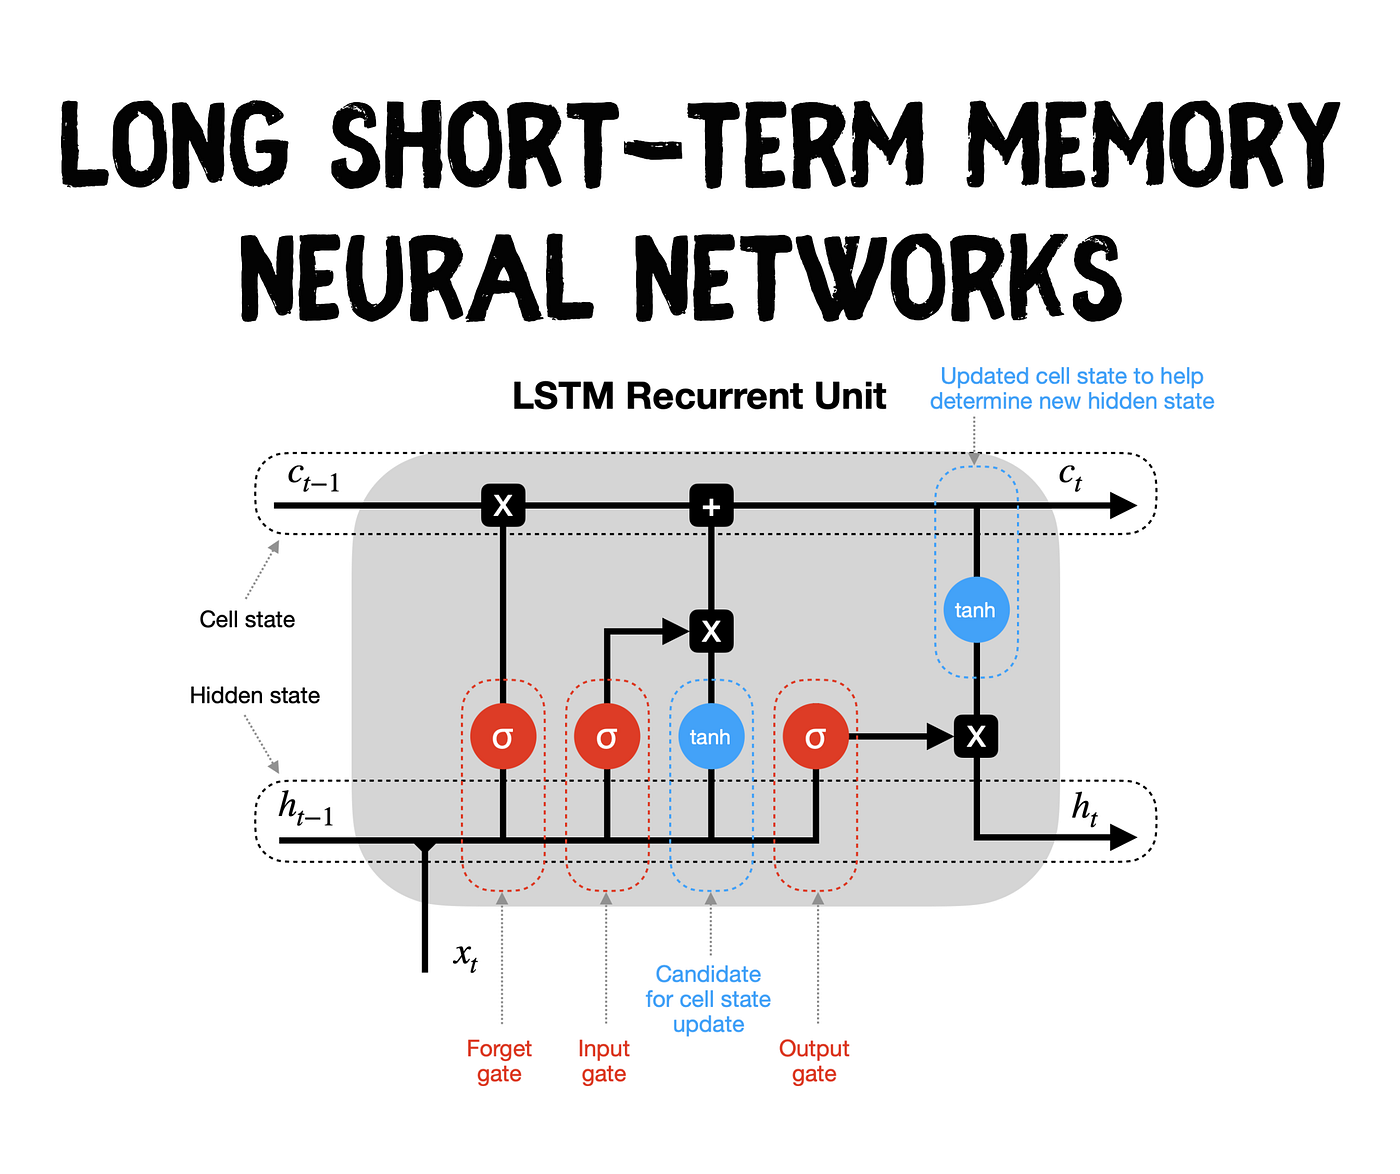
\includegraphics[width=0.8\textwidth]{lstm.png}
		\caption{Algoritma LSTM \textit{(source: \cite{SaulDobilas})}}
	\end{figure}
	LSTM memiliki gerbang \textit{(gate)} yang lebih rumit dibanding algoritma yang lain yang menyebabkan LSTM memiliki tingkat kemampuan akurasi yang jauh lebih tinggi dibanding algoritma lainnya. Namun LSTM memiliki kekurangan yaitu pada tahap \textit{(training)} / proses latihan yang lebih lama. berikut merupakan gerbang-gerbang yang digunakan dalam algoritma LSTM.
	Berikut merupakan langkah-langkah latihan yang dilakukan oleh LSTM:
	\begin{figure}[H]
		\centering
		\begin{subfigure}[b]{0.45\textwidth}
			\centering
			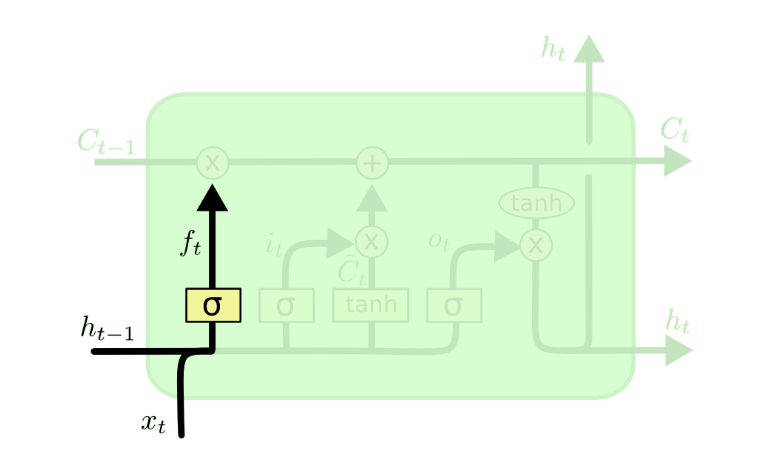
\includegraphics[width=\textwidth]{step1.png}
			% \caption{Forget Gate}
		\end{subfigure}
		\hfill
		\begin{subfigure}[b]{0.5\textwidth}
			\centering
			\[
				f_t = \sigma \left( W_f \cdot \begin{bmatrix} h_{t-1},x_t \end{bmatrix} + b_f \right) ..... (1)
			\]
		\end{subfigure}
		\caption{Forget Gate dengan rumusnya}
	\end{figure}
	Langkah pertama pada proses latihan LSTM adalah menentukan informasi apa yang akan diteruskan ke layer selanjutnya/\textit{cell layer}. Layer ini menggunakan rumus \textit{sigmoid} untuk menentukan hasil antara 0 dengan 1

	\begin{figure}[H]
		\centering
		\begin{subfigure}[b]{0.45\textwidth}
			\centering
			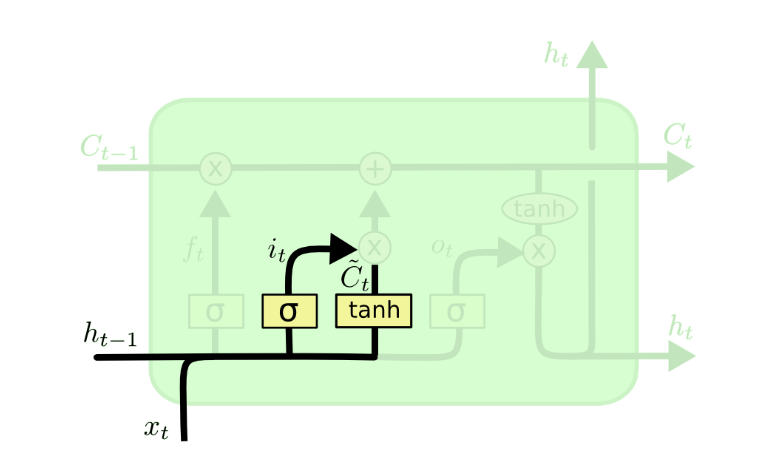
\includegraphics[width=\textwidth]{step2.png} % Replace with your image file
			% \caption{Input Gate}
		\end{subfigure}
		\hfill
		\begin{subfigure}[b]{0.5\textwidth}
			\centering
			\[
				i_t = \sigma \left( W_f \cdot \begin{bmatrix} h_{t-1},x_t \end{bmatrix} + b_i \right)  ..... (2)
			\]
			\[
				C_t = \tanh \left( W_C \cdot \begin{bmatrix} h_{t-1},x_t \end{bmatrix} + b_C \right) ..... (3)
			\]
		\end{subfigure}
		\caption{Input Gate dengan rumusnya}
	\end{figure}
	Selanjutnya adalah proses \textit{Input Gate}, yaitu proses untuk menambahkan informasi baru ke \textit{Cell Layer}. Dalam layer ini juga memutuskan informasi baru apa yang akan disimpan kedalam \textit{Cell State}

	\begin{figure}[H]
		\centering
		\begin{subfigure}[b]{0.45\textwidth}
			\centering
			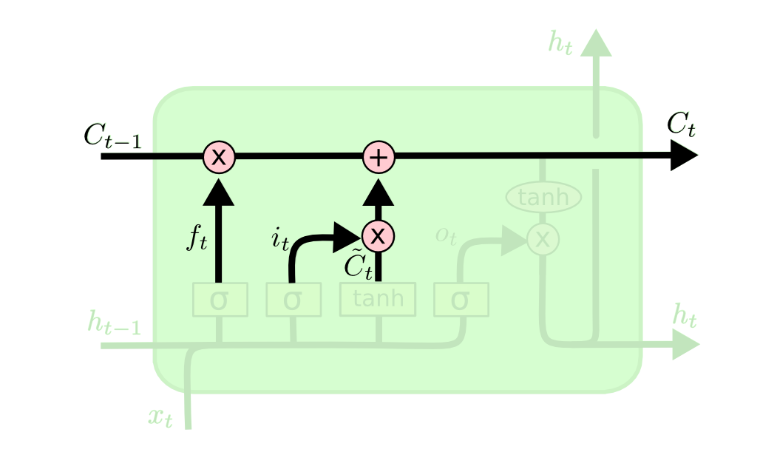
\includegraphics[width=\textwidth]{step3.png}
			% \caption{Pembaruan Cell State}
		\end{subfigure}
		\hfill
		\begin{subfigure}[b]{0.5\textwidth}
			\centering
			\[
				f_t = \sigma \left( W_f \cdot \begin{bmatrix} h_{t-1},x_t \end{bmatrix} + b_f \right) ..... (4)
			\]
		\end{subfigure}
		\caption{Pembaruan Cell State dengan rumusnya}
	\end{figure}
	Selanjutnya adalah proses pembaruan \textit{Cell State}. Informasi yang sudah dipilih dalam layer sebelumnya akan dijadikan data yang baru dan data yang lama akan dihapus. Hal ini memastikan bahwa LSTM akan selalu bekerja dengan informasi yang relevan untuk menghasilkan prediksi yang akurat.

	\begin{figure}[H]
		\centering
		\begin{subfigure}[b]{0.45\textwidth}
			\centering
			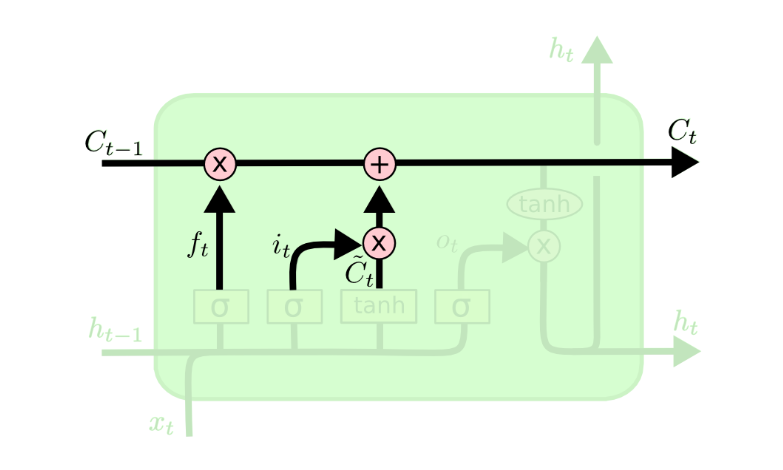
\includegraphics[width=\textwidth]{step4.png}
			% \caption{Output Gate}
		\end{subfigure}
		\hfill
		\begin{subfigure}[b]{0.5\textwidth}
			\centering
			\[
				f_t = \sigma \left( W_f \cdot \begin{bmatrix} h_{t-1},x_t \end{bmatrix} + b_f \right) ..... (5)
			\]
		\end{subfigure}
		\caption{Output Gate dengan rumusnya}
	\end{figure}
	Langkah terakhir adalah proses \textit{Output Gate}, yaitu proses menentukan informasi apa yang akan dihasilkan sebagai output. Proses ini memiliki 3 proses penyaringan sebelum menjadi sebuah output, yaitu Pemfilteran awal dengan sigmoid layer, Normalisasi dengan fungsi tanh dan Kombinasi hasil (\cite{Christopher}).

\end{subs}

\textbf{\section{Studi Literatur}}

\begin{center}
  \centering
	\begin{longtable}{| m{1cm} | m{3cm}| p{8cm} |}
		\hline
		\multicolumn{1}{|c|}{\textbf{No.}} & \multicolumn{1}{c|}{\textbf{Kriteria}} & \multicolumn{1}{c|}{\textbf{Isi}}                                                                                                                                                                                                                                                                                                                                                                                                             \\

    \hline
		\endfirsthead

    \hline
    \endhead

    \hline
		\endfoot

		\hline
		\endlastfoot

		\multirow[t]{6}{*}{1.}             & Nama Peneliti                          & \cite{pipin2023prediksi}                                                                                                                                                                                                                                                                                                                                                                                                                                                                                                                                                                                                                                                                                                                                                                                                                                                                                                                                                                                                                                                                                                                                                                                                                                                                                                                                                                                                                                                                                                                                                                                                                                                                                                                                                                                                                                                                                                                                                                                                                                                                                                                                                                                                                                                                                                                                                                                                                                                                                                                                                                                                                                           \\         
		\cline{2-3}
		                                   & Judul Penelitian                       & Prediksi Saham Menggunakan Recurrent Neural Network (RNN-LSTM) dengan Optimasi Adaptive Moment Estimation                                                                                                                                                                                                                                                                                                                                     \\
		\cline{2-3}
		                                   & Permasalahan dan Tujuan                & Penelitian ini bertujuan untuk mengembangkan model prediksi harga saham dengan menggunakan algoritma LSTM, dengan tujuan untuk meningkatkan akurasi prediksi harga saham di pasar Indonesia.                                                                                                                                                                                                                                                  \\
		\cline{2-3}
		                                   & Metode                                 & Penelitian ini menggunakan data historis harga saham perusahaan yang terdaftar di Bursa Efek Indonesia (BEI). Model LSTM dikembangkan untuk mengolah data time series dan digunakan untuk memprediksi harga saham di masa depan.                                                                                                                                                                                                              \\
		\cline{2-3}
		                                   & Hasil                                  & Hasil penelitian menunjukkan bahwa model LSTM memiliki akurasi yang lebih baik dibandingkan dengan model RNN dalam memprediksi harga saham, dengan MAPE (Mean Absolute Percentage Error) yang lebih rendah.                                                                                                                                                                                                                                   \\
		\cline{2-3}
		                                   & Kelebihan dan Kekurangan               & Kelebihan: Penelitian ini berhasil menunjukkan bahwa LSTM dapat menghasilkan prediksi yang lebih akurat dibandingkan dengan metode lain, terutama dalam memproses data yang bersifat non-linear dan kompleks. \newline Kekurangan: Penelitian ini hanya membandingkan dua model (LSTM dan RNN) tanpa mempertimbangkan algoritma lain yang mungkin lebih sesuai untuk jenis data tertentu, seperti model berbasis transformator (Transformer). \\

    \hline
		\multirow[t]{6}{*}{2.}             & Nama Peneliti                          & \cite{moghar2020stock} \\
		\cline{2-3}
		                                   & Judul Penelitian                       & Stock Market Prediction Using LSTM Recurrent Neural Network \\
		\cline{2-3}
		                                   & Permasalahan dan Tujuan                & Penelitian ini membahas tantangan dalam memprediksi harga saham, terutama karena volatilitas tinggi dan pola non-linear dalam data. Tujuannya adalah mengevaluasi efektivitas model LSTM dalam memprediksi harga saham berdasarkan data historis. \\
		\cline{2-3}
		                                   & Metode                                 & Menggunakan data historis harga saham, model LSTM diimplementasikan dengan berbagai parameter untuk menangkap pola non-linear. Evaluasi dilakukan terhadap performa model dalam memprediksi harga saham masa depan. \\
		\cline{2-3}
		                                   & Hasil                                  & LSTM memberikan hasil yang lebih akurat dibandingkan model tradisional seperti ARIMA, khususnya dalam menangkap pola volatilitas saham. \\
		\cline{2-3}
		                                   & Kelebihan dan Kekurangan               & Kelebihan: Efektif dalam menangani data time series dengan pola kompleks dan non-linear.\newline Kekurangan: Bergantung pada parameter model yang harus dioptimalkan untuk hasil terbaik. \\

    \hline
		\multirow[t]{6}{*}{3.}             & Nama Peneliti                          & \cite{alim2023pemodelan} \\
		\cline{2-3}
		                                   & Judul Penelitian                       & Pemodelan Time Series Data Saham LQ45 dengan Algoritma LSTM, RNN, dan ARIMA \\
		\cline{2-3}
		                                   & Permasalahan dan Tujuan                & Penelitian ini bertujuan membandingkan performa algoritma LSTM, RNN, dan ARIMA dalam memprediksi harga saham LQ45 untuk menentukan model yang paling akurat. \\
		\cline{2-3}
		                                   & Metode                                 & Dataset saham LQ45 diproses untuk membangun model LSTM, RNN, dan ARIMA. Evaluasi dilakukan menggunakan metrik akurasi seperti MSE (Mean Squared Error) dan MAE (Mean Absolute Error). \\
		\cline{2-3}
		                                   & Hasil                                  & LSTM memberikan hasil terbaik dalam memprediksi harga saham dibandingkan RNN dan ARIMA karena kemampuannya menangkap pola jangka panjang dan non-linear. \\
		\cline{2-3}
		                                   & Kelebihan dan Kekurangan               & Kelebihan: Memberikan perbandingan kinerja model berbasis time series.\newline Kekurangan: Fokus hanya pada data LQ45 tanpa mempertimbangkan pengaruh faktor fundamental saham.\\

    \hline
		\multirow[t]{6}{*}{4.}             & Nama Peneliti                          & \cite{sofi2021perbandingan} \\
		\cline{2-3}
		                                   & Judul Penelitian                       & Perbandingan Algoritma Linear Regression, LSTM, dan GRU dalam Memprediksi Harga Saham dengan Model Time Series \\
		\cline{2-3}
		                                   & Permasalahan dan Tujuan                & Penelitian ini bertujuan untuk membandingkan performa algoritma Linear Regression, LSTM, dan GRU dalam memprediksi harga saham menggunakan data time series. \\
		\cline{2-3}
		                                   & Metode                                 & Dataset harga saham historis diproses untuk melatih model Linear Regression, LSTM, dan GRU. Kinerja model dibandingkan menggunakan metrik RMSE dan R-squared. \\
		\cline{2-3}
		                                   & Hasil                                  & LSTM dan GRU menunjukkan performa yang lebih unggul dibandingkan Linear Regression, dengan LSTM memberikan akurasi terbaik dalam menangkap pola non-linear. \\
		\cline{2-3}
		                                   & Kelebihan dan Kekurangan               & Kelebihan: Memberikan analisis komparatif yang kuat antara algoritma time series populer.\newline Kekurangan: Tidak mengeksplorasi dampak hyperparameter tuning pada performa model.\\

    \hline
		\multirow[t]{6}{*}{5.}             & Nama Peneliti                          & \cite{chairurrachman2022penerapan} \\
		\cline{2-3}
		                                   & Judul Penelitian                       & Penerapan Long Short-Term Memory pada Data Time Series untuk Prediksi Harga Saham PT Indofood CBP Sukses Makmur Tbk (ICBP) \\
		\cline{2-3}
		                                   & Permasalahan dan Tujuan                & Penelitian ini bertujuan mengevaluasi efektivitas LSTM dalam memprediksi harga saham perusahaan tertentu, dalam hal ini PT ICBP. Fokus utama adalah menangkap pola data historis saham yang kompleks. \\
		\cline{2-3}
		                                   & Metode                                 & Data historis saham PT ICBP diproses dan dimasukkan ke dalam model LSTM yang telah dioptimalkan melalui pengaturan hyperparameter. Evaluasi dilakukan dengan membandingkan akurasi prediksi dengan data aktual. \\
		\cline{2-3}
		                                   & Hasil                                  & LSTM berhasil menangkap pola harga saham PT ICBP dengan akurasi yang cukup tinggi. \\
		\cline{2-3}
		                                   & Kelebihan dan Kekurangan               & Kelebihan: Fokus pada perusahaan spesifik, memungkinkan analisis yang mendalam dan terarah.\newline Kekurangan: Tidak memperhatikan pengaruh faktor eksternal seperti kondisi pasar dan ekonomi global. \\

    \hline
    \multirow[t]{6}{*}{6.}             & Nama Peneliti                          & \cite{julian2021peramalan} \\
		\cline{2-3}
		                                   & Judul Penelitian                       & Peramalan Harga Saham Pertambangan pada Bursa Efek Indonesia Menggunakan Long Short Term Memory (LSTM). \\
		\cline{2-3}
		                                   & Permasalahan dan Tujuan                & Penelitian ini membahas penerapan LSTM untuk memprediksi harga saham sektor pertambangan di Bursa Efek Indonesia (BEI). Tujuannya adalah mengevaluasi akurasi prediksi menggunakan LSTM dibandingkan pendekatan lainnya. \\
		\cline{2-3}
		                                   & Metode                                 & Data historis saham sektor pertambangan diolah melalui tahapan preprocessing. Model LSTM dibangun untuk prediksi, dan performanya dibandingkan dengan metode lain menggunakan metrik akurasi seperti RMSE. \\
		\cline{2-3}
		                                   & Hasil                                  & LSTM memberikan akurasi terbaik dibandingkan metode tradisional dalam memprediksi saham sektor pertambangan. \\
		\cline{2-3}
		                                   & Kelebihan dan Kekurangan               & Kelebihan: Memanfaatkan algoritma canggih untuk sektor industri spesifik.\newline Kekurangan: Terbatas pada sektor pertambangan, sehingga kurang relevan untuk sektor lain. \\
	\end{longtable}
\end{center}
\addlongtabletolist{Studi Literatur}


% chapter 3
\setcounter{chapter}{3}
\setcounter{section}{0}
\chapter*{\textbf{BAB III \\ METODOLOGI PENELITIAN}}
\addcontentsline{toc}{chapter}{BAB III}
\addcontentsline{toc}{chapter}{METODOLOGI PENELITIAN}
\textbf{\section{Lokasi Penelitian}}
\indent

Dikarenakan data yang akan digunakkan dalam penelitian ini dapat diperoleh dari melalui internet, maka penelitian ini dapat dilakukan dimana saja atau secara daring. Dalam penelitian ini, peneliti menggunakan data yang bersumber pada \href{https://finance.yahoo.com}{yahoo finance}. Alasan menggunakan yahoo finance? karena yahoo finance menyediakan data historis saham yang sangatlah lengkap bukan hanya saham Indonesia saja, melainkan saham international juga. Selain itu data yang disediakan oleh yahoo finance memiliki isi yang sangat relevan bahkan mencakup \textit{OHLC (Open, High, Low, Close)}, volume, serta indikator teknikal lainnya.

\begin{figure}[H]
	\centering
	
\includegraphics[width=0.5\textwidth]{yahoo_finance.png}
	\caption{Logo Yahoo Finance}
\end{figure}

% TODO: lengkapi lagi
Yahoo Finance adalah platform yang sering digunakan untuk data keuangan dan memiliki banyak keunggulan yang membuatnya pilihan ideal untuk analisis harga saham, terutama ketika menggunakan data historis. Berikut alasan mengapa Yahoo Finance sangatlah digunakan dalam penelitian ini:
\begin{itemize}
  	\item \textit{Gratis}: Yahoo Finance menyediakan data yang gratis dan dapat digunakan untuk penelitian tanpa harus membayar biaya.
	\item \textit{Data Historis}: Yahoo Finance menyediakan data historis saham yang sangatlah lengkap dan dapat digunakan untuk analisis harga saham. Data ini dapat dikumpulkan dari berbagai sumber seperti Yahoo Finance, Yahoo Finance Indonesia, dan Yahoo Finance Global.
	\item \textit{Relevansi}: Data yang disediakan oleh Yahoo Finance memiliki isi yang sangat relevan dan dapat digunakan untuk analisis harga saham. Data ini juga memiliki indikator teknikal yang dapat digunakan untuk menganalisis data saham.
	\item \textit{Integrasi dengan python}: Yahoo Finance dapat diakses menggunakan \textit{python} dengan menggunakan \textit{library} yaitu \textit{`yfinance`}. Dengan hal ini penelitian ini akan dapat mudah dalam melakukan proses preprocessing data sebelum digunakan pada model machine learning seperti LSTM.
\end{itemize}

\textbf{\section{Waktu Penelitian}}

Penelitian ini dilaksanakan pada bulan september hingga november dan dijadwalkan untuk berlangsung pada tahun 2024. Durasi tersebut dipilih untuk memastikan data yang akan dikumpulkan relevan dan juga komprehensif dengan penelitian ini serta menyediakan cukup waktu untuk melakukan pengamatan dan analisis data yang akan dihasilkan.


\textbf{\section{Penentuan Subjek Penelitian}}

% TODO: lengkapi lagi
Subjek penelitian ini merupakan saham-saham yang terdaftar di Bursa Efek Indonesia (BEI) terutama saham LQ45. Penelitian ini menggunakan data saham indeks yang tergolong utama yaitu LQ45 dengan rentang waktu 5-10 tahun terakhir. Data saham ini akan di analisis dengan menggunakan algoritma \textit{Long Short-Term Memory (LSTM)} yang merupakan bagian dari \textit{Recurrent Neural Network (RNN)}, untuk memprediksi pergerakan harga saham berdasarkan pola data sekuensial. Selain itu, hasil prediksi dari model LSTM akan dimanfaatkan dalam sistem pendukung keputusan investasi untuk memberikan rekomendasi terkait aksi investasi, seperti membeli, menjual, atau menahan saham, sehingga penelitian ini tidak hanya fokus pada aspek teknis tetapi juga pada penerapannya dalam konteks pengambilan keputusan di dunia nyata.


\textbf{\section{Fokus Penelitian}}

% TODO: lengkapi lagi
Fokus dari penelitian ini adalah untuk menganalisis pergerakan dari harga saham di Indonesia terutama saham LQ45 yang terdaftar di Bursa Efek Indonesia (BEI) dengan menggunakan algoritma \textit{Long Short-Term Memory (LSTM)} sebagai metode prediksi berbasis data historis. Penelitian ini dilakukan guna mengidentifikasi pola pergerakan harga saham dari data historis yang berguna untuk menghasilkan prediksi yang dapat mendukung pengambilan keputusan investasi. Selain itu, penelitian ini juga berfokus pada pengembangan sistem pendukung keputusan investasi berbasis teknologi yang memanfaatkan hasil prediksi model LSTM untuk memberikan rekomendasi strategis seperti membeli, menjual, atau menahan saham. Dengan demikian, penelitian ini menggabungkan pendekatan teknis berbasis algoritma kecerdasan buatan dengan aplikasi praktis dalam konteks investasi di pasar saham Indonesia.


\textbf{\section{Sumber Data}}
Sumber data yang digunakan dalam penelitian ini adalah data saham indeks yang tergolong utama yaitu LQ45 dengan rentang waktu 5-10 tahun terakhir yang akan diperoleh dari \href{https://finance.yahoo.com}{yahoo finance}. Data yang akan diperoleh meliputi:
\begin{itemize}
	\item \textit{High}: Harga saham tertinggi
	\item \textit{Low}: Harga saham terendah
	\item \textit{Close}: Harga saham terakhir/penutupan
	\item \textit{Volume}: Volume saham
\end{itemize}

Data ini akan diunduh dalam format \textit{CSV} untuk mempermudah proses analisis menggunakan perangkat lunak seperti Python dengan bantuan library seperti yfinance. Selain Yahoo Finance, jika diperlukan, data tambahan dapat diperoleh dari sumber alternatif seperti laporan tahunan perusahaan terkait atau data dari Bursa Efek Indonesia (BEI).


\textbf{\section{Teknik Pengumpulan Data}}

% TODO: tambahkan lagi
Teknik penelitian yang akan digunakan dalam penelitian ini adalah studi literatur, yang berfokus pada pengumpulan dan analisis sumber-sumber sekunder yang relevan untuk mendalami topik analisis pergerakan harga saham menggunakan algoritma Long Short-Term Memory (LSTM). Studi literatur ini bertujuan untuk mendapatkan pemahaman yang lebih dalam tentang berbagai konsep yang terkait dengan penelitian, termasuk teori dasar mengenai saham, metode analisis saham seperti analisis fundamental dan teknikal, serta penerapan algoritma deep learning dalam prediksi harga saham.

Proses pertama dalam studi literatur adalah mengidentifikasi dan mengumpulkan berbagai referensi yang relevan, baik berupa buku, artikel ilmiah, jurnal, laporan riset, dan publikasi terkait lainnya yang membahas tentang analisis saham, kecerdasan buatan, serta aplikasi LSTM dalam data keuangan. Sumber-sumber ini akan digunakan untuk menggali teori dasar dan konsep-konsep yang berkaitan dengan analisis teknikal dan prediksi harga saham, serta memberikan gambaran tentang penggunaan algoritma LSTM dalam konteks pasar saham.

Setelah pengumpulan sumber, langkah selanjutnya adalah melakukan analisis terhadap literatur yang ada untuk mengidentifikasi temuan-temuan penting dan tren yang muncul dalam penelitian sebelumnya. Fokus utama adalah untuk membandingkan berbagai pendekatan yang telah digunakan dalam analisis saham, baik yang berbasis analisis fundamental, teknikal, maupun yang menggunakan teknologi kecerdasan buatan seperti deep learning dan LSTM. Selain itu, penelitian ini juga akan mengidentifikasi kelebihan dan kekurangan dari berbagai metode yang ada, serta melihat sejauh mana penggunaan LSTM dapat meningkatkan akurasi prediksi harga saham dibandingkan dengan algoritma lain seperti Recurrent Neural Networks (RNN).

Hasil dari studi literatur ini diharapkan dapat memberikan wawasan yang lebih jelas mengenai penerapan LSTM dalam memprediksi pergerakan harga saham di Indonesia, khususnya saham-saham yang terdaftar dalam LQ45. Studi literatur ini juga akan memberikan dasar teoretis untuk penelitian selanjutnya yang akan melibatkan pengumpulan dan analisis data harga saham historis untuk menguji efektivitas LSTM dalam prediksi harga saham.


\textbf{\section{Tahapan Penelitian}}
Dalam melaksanakan penelitian ini, terdapat beberapa tahapan penting yang harus dilakukan secara sistematis untuk mencapai hasil yang optimal. Setiap tahapan dirancang untuk memastikan bahwa proses penelitian berjalan dengan terstruktur dan menghasilkan keluaran yang valid. Penelitian ini dimulai dari pengumpulan data yang relevan, diikuti dengan proses pengolahan data untuk memastikan data siap digunakan dalam analisis lebih lanjut. Setelah itu, dataset dibagi untuk melatih dan menguji model yang dipilih. Pemilihan model dilakukan dengan mempertimbangkan tujuan penelitian dan karakteristik data yang digunakan.

Tahapan berikutnya adalah mengevaluasi performa model berdasarkan metrik tertentu untuk memastikan hasil yang dihasilkan memiliki tingkat keakuratan yang dapat diterima. Terakhir, hasil dari proses ini dianalisis lebih mendalam dan divisualisasikan untuk memberikan pemahaman yang lebih intuitif dan mudah dipahami. Berikut ini adalah penjelasan rinci untuk setiap tahapan penelitian yang telah dilakukan.

% TODO: lengkapi
\begin{subs}
	\subsection{Pengumpulan Data}
	\indent

	Tahapan pengumpulan data dalam penelitian ini dilakukan untuk mendapatkan data historis pergerakan harga saham pada indeks LQ45 yang akan digunakan sebagai basis analisis prediksi. Proses pengumpulan data dilakukan dengan langkah-langkah sebagai berikut:
	\begin{enumerate}
		\item Pemilihan Emiten \\
		      Data yang dikumpulkan hanya mencakup saham-saham dari perusahaan yang masuk dalam indeks LQ45 pada periode tertentu. Emiten-emiten ini dipilih karena mereka mewakili perusahaan-perusahaan yang memiliki likuiditas tinggi dan stabilitas keuangan yang relatif baik.

		\item Jenis Data yang Dikumpulkan \\
		      Data historis yang dikumpulkan meliputi:
		      \begin{itemize}
			      \item Harga pembukaan (opening price)
			      \item Harga penutupan (closing price)
			      \item Harga tertinggi (high price)
			      \item Harga terendah (low price)
			      \item Volume perdagangan (trading volume)
		      \end{itemize}

		\item Platform Pengumpulan Data \\
		      Data diperoleh melalui fitur pengunduhan yang disediakan oleh Yahoo Finance. Platform ini dipilih karena:
		      \begin{itemize}
			      \item Menyediakan data historis secara gratis dan mudah diakses.
			      \item Format data yang dapat diunduh (seperti CSV) memudahkan proses analisis lebih lanjut.
		      \end{itemize}

		\item Proses Pengambilan Data \\
		      \renewcommand{\labelenumi}{\alph{enumi}.}
		      \begin{enumerate}
			      \item Melihat data yang tersedia pada \href{https://finance.yahoo.com}{Yahoo Finance}
			      \item Memasukkan kode saham dari emiten yang terdaftar dalam indeks LQ45.
			      \item Menginstall python untuk melakukan analisis serta pengambilan data.
			      \item Menginstall library yfinance untuk melakukan pengambilan data.
			      \item Menulis kode python untuk mengunduh dataset dari yahoo finance dengan memasukkan kode saham sesuai kode pada saham LQ45.
		      \end{enumerate}

		\item Validasi dan Verifikasi Data \\
		      Setelah data dikumpulkan, dilakukan proses validasi untuk memastikan data yang diperoleh sesuai dengan kebutuhan penelitian. Langkah-langkah validasi meliputi:
		      \begin{itemize}
			      \item Memeriksa konsistensi data (tidak ada duplikasi atau nilai yang hilang).
			      \item Memastikan kelengkapan data untuk setiap emiten yang dipilih.
			      \item Menyelaraskan format data agar kompatibel dengan alat analisis, seperti Python dan Pandas.
		      \end{itemize}


	\end{enumerate}

	\subsection{Preprocessing Data}
	\renewcommand{\labelenumi}{\alph{enumi}.}
	\indent

	Preprocessing data adalah tahap untuk membersihkan, mengubah, dan mempersiapkan data agar sesuai untuk digunakan dalam model machine learning. Langkah ini penting untuk memastikan data yang digunakan bersih, relevan, dan terstruktur.
	\begin{enumerate}
		\item Cleaning Data
		      Cleaning data atau pembersihan data merupakan sebuah proses yang sangat penting dalam penelitian untuk memisahkan data yang kotor seperti data yang hilang dan juga menghapus data kolom yang tidak relevan.
		\item Normalization Data
		      Normalization data adalah proses untuk mengatur data yang bervariasi antara satu sama lain menjadi data yang relatif yang sama. Proses ini dapat dilakukan dengan menggunakan metode-metode yang berbeda seperti min-max scaling, z-score, dan standarisasi. Data akan diubah ke dalam rentang 0 hingga 1 menggunakan metode MinMaxScaler untuk meningkatkan efisiensi model
		      \begin{lstlisting}
            import numpy as np
            from sklearn.preprocessing import MinMaxScaler

            data = np.array([1, 2, 3, 4, 5])
            scaler = MinMaxScaler()
            normalized_data = scaler.fit_transform(data.reshape(-1, 1))
            print(normalized_data)
        \end{lstlisting}
		\item Feature Engineering
		      Membuat fungsi untuk membagi data menjadi sekumpulan urutan waktu (sequences) dan label
		      \begin{lstlisting}
            def create_dataset(dataset, sequence_length=50):
            x, y = [], []
            for i in range(len(dataset) - sequence_length):
            x.append(dataset[i:i + sequence_length])
            y.append(dataset[i + sequence_length])
            return np.array(x), np.array(y)

            x, y = create_dataset(normalized_data)
          \end{lstlisting}
	\end{enumerate}

	\subsection{Pembagian Dataset}
	\indent

	Dalam penelitian ini, dataset akan dibagi menjadi dua set data yaitu, training data dan testing data. Training data digunakan untuk membuat model dan testing data digunakan untuk mengevaluasi model yang telah dibuat.
	Dalam penelitian ini data yang digunakan untuk proses latihan sebesar 80\% dan untuk validasi sebesar 20\%.
	\begin{lstlisting}
    train_size = int(len(x) * 0.8)
    x_train, x_test = x[:train_size], x[train_size:]
    y_train, y_test = y[:train_size], y[train_size:]
  \end{lstlisting}

	\subsection{Pemilihan Model}
	\indent

	Pemilihan model dan pelatihan bertujuan untuk memilih algoritma yang sesuai dengan kebutuhan penelitian. Pelatihan model dilakukan dengan memberikan data latih sehingga model dapat belajar pola dari data tersebut.
	Di Penelitian ini, model yang akan digunakan adalah LSTM. dikarenakan LSTM memiliki kemampuan untuk menganalisis data urutan waktu dan memprediksi data masa depan yang jauh lebih akurat dibanding dengan model tradisional seperti ARIMA dan model-model lainnya.

	\subsection{Evaluasi Model}
	\indent

	Evaluasi model adalah proses untuk mengukur kinerja model yang telah dilatih menggunakan metrik tertentu. Dalam penelitian ini, evaluasi dilakukan dengan membandingkan hasil prediksi dengan data aktual menggunakan Loss Function, Mean Squared Error (MSE) dan Mean Absolute Error (MAE).
	\begin{itemize}
		\item Mean Squared Error (MSE)
		      MSE adalah salah satu metrik yang paling umum digunakan untuk mengevaluasi model regresi, termasuk model LSTM. Metrik ini menghitung rata-rata dari kuadrat selisih antara nilai yang diprediksi dan nilai yang sebenarnya. MSE lebih sensitif terhadap kesalahan yang lebih besar karena setiap kesalahan dipangkatkan dua kali, sehingga kesalahan besar akan memberikan dampak yang lebih besar pada hasilnya.
		\item Mean Absolute Error (MAE)
		      MAE adalah metrik yang menghitung rata-rata dari nilai absolut perbedaan antara nilai yang diprediksi dan nilai yang sebenarnya. Berbeda dengan MSE, MAE tidak memberikan penalti yang lebih besar pada kesalahan besar, sehingga lebih robust terhadap outlier.
		\item Loss Function
		      Loss function adalah fungsi yang digunakan oleh model selama proses pelatihan untuk mengukur seberapa baik atau buruk prediksi model dibandingkan dengan nilai yang sebenarnya. Loss function bertujuan untuk mengoptimalkan kinerja model dengan meminimalkan nilai loss function selama pelatihan.

		      Pada model LSTM, loss function yang sering digunakan adalah Mean Squared Error (MSE), tetapi bisa juga menggunakan Mean Absolute Error (MAE) atau jenis loss function lainnya tergantung pada jenis model dan masalah yang dihadapi. Selama pelatihan, model LSTM mencoba meminimalkan nilai loss function melalui algoritma optimasi seperti Adam, SGD, atau lainnya.
	\end{itemize}

	\subsection{Analisis Hasil \& Visualisasi}
	Tahap ini bertujuan untuk memahami hasil yang diperoleh dari model dan menyajikannya dalam bentuk yang mudah dipahami, seperti grafik atau tabel.
	\begin{figure}[H]
		\centering
		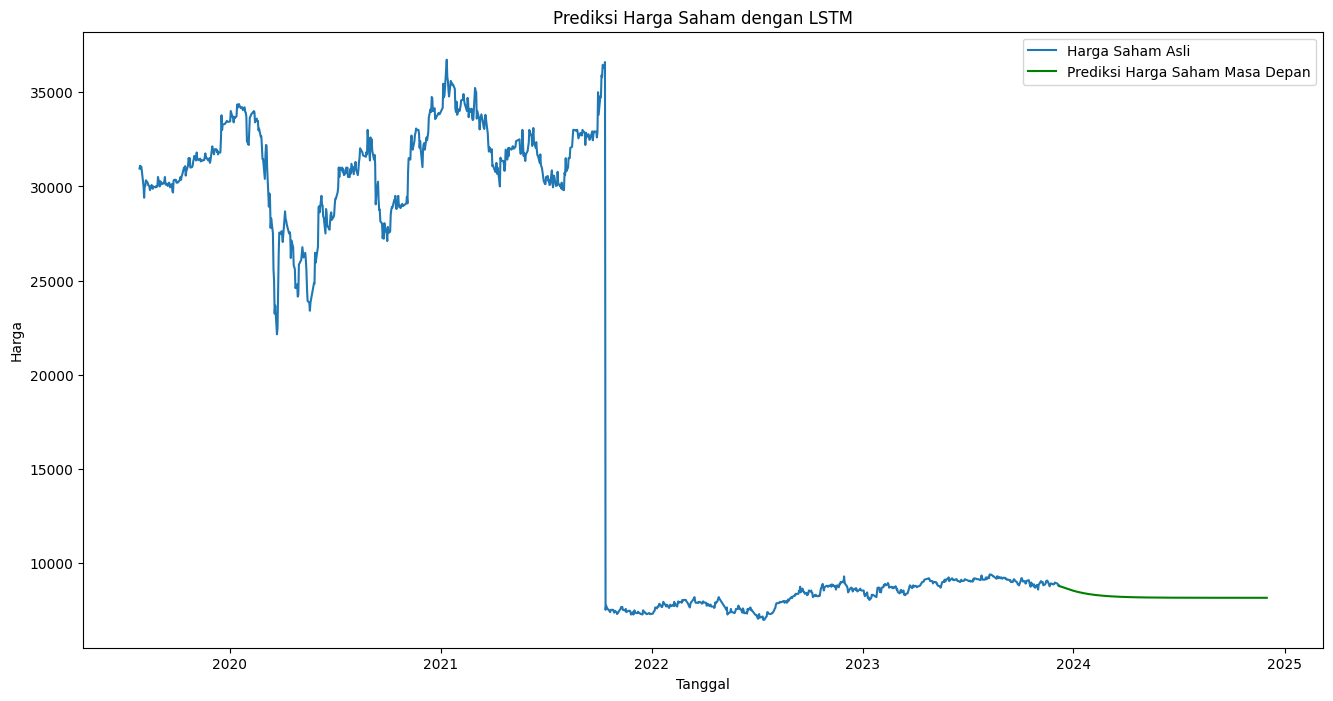
\includegraphics[width=0.8\textwidth]{hasil_analisis.png}
		\caption{Grafik hasil analisis}
    \addimagetolist{Grafik hasil analisis}{hasil_analisis.png}
	\end{figure}


\end{subs}


% insert bibliography
\printbibliography[title=\textbf{Daftar Pustaka}]

\end{document}
